\documentclass{ximera}

\usepackage{epsfig}

\graphicspath{
  {./}
  {figures/}
}


\usepackage{morewrites}

%\newcounter{ccounter}
%\setcounter{ccounter}{1}
%\newcommand{\Chapter}[1]{\setcounter{chapter}{\arabic{ccounter}}\chapter{#1}\addtocounter{ccounter}{1}}

%\newcommand{\section}[1]{\section{#1}\setcounter{thm}{0}\setcounter{equation}{0}}

%\renewcommand{\theequation}{\arabic{chapter}.\arabic{section}.\arabic{equation}}
%\renewcommand{\thefigure}{\arabic{chapter}.\arabic{figure}}
%\renewcommand{\thetable}{\arabic{chapter}.\arabic{table}}

%\newcommand{\Sec}[2]{\section{#1}\markright{\arabic{ccounter}.\arabic{section}.#2}\setcounter{equation}{0}\setcounter{thm}{0}\setcounter{figure}{0}}

\newcommand{\Sec}[2]{\section{#1}}

\setcounter{secnumdepth}{2}
%\setcounter{secnumdepth}{1} 

%\newcounter{THM}
%\renewcommand{\theTHM}{\arabic{chapter}.\arabic{section}}

\newcommand{\trademark}{{R\!\!\!\!\!\bigcirc}}
%\newtheorem{exercise}{}

\newcommand{\dfield}{{\sf dfield9}}
\newcommand{\pplane}{{\sf pplane9}}

\newcommand{\EXER}{\section*{Exercises}}%\vspace*{0.2in}\hrule\small\setcounter{exercise}{0}}
\newcommand{\CEXER}{}%\vspace{0.08in}\begin{center}Computer Exercises\end{center}}
\newcommand{\TEXER}{} %\vspace{0.08in}\begin{center}Hand Exercises\end{center}}
\newcommand{\AEXER}{} %\vspace{0.08in}\begin{center}Hand Exercises\end{center}}

% BADBAD: \newcommand{\Bbb}{\bf}

\newcommand{\R}{\mbox{$\Bbb{R}$}}
\newcommand{\C}{\mbox{$\Bbb{C}$}}
\newcommand{\Z}{\mbox{$\Bbb{Z}$}}
\newcommand{\N}{\mbox{$\Bbb{N}$}}
\newcommand{\D}{\mbox{{\bf D}}}
\usepackage{amssymb}
%\newcommand{\qed}{\hfill\mbox{\raggedright$\square$} \vspace{1ex}}
%\newcommand{\proof}{\noindent {\bf Proof:} \hspace{0.1in}}

\newcommand{\setmin}{\;\mbox{--}\;}
\newcommand{\Matlab}{{M\small{AT\-LAB}} }
\newcommand{\Matlabp}{{M\small{AT\-LAB}}}
\newcommand{\computer}{\Matlab Instructions}
\newcommand{\half}{\mbox{$\frac{1}{2}$}}
\newcommand{\compose}{\raisebox{.15ex}{\mbox{{\scriptsize$\circ$}}}}
\newcommand{\AND}{\quad\mbox{and}\quad}
\newcommand{\vect}[2]{\left(\begin{array}{c} #1_1 \\ \vdots \\
 #1_{#2}\end{array}\right)}
\newcommand{\mattwo}[4]{\left(\begin{array}{rr} #1 & #2\\ #3
&#4\end{array}\right)}
\newcommand{\mattwoc}[4]{\left(\begin{array}{cc} #1 & #2\\ #3
&#4\end{array}\right)}
\newcommand{\vectwo}[2]{\left(\begin{array}{r} #1 \\ #2\end{array}\right)}
\newcommand{\vectwoc}[2]{\left(\begin{array}{c} #1 \\ #2\end{array}\right)}



\newcommand{\inv}{^{-1}}
\newcommand{\CC}{{\cal C}}
\newcommand{\CCone}{\CC^1}
\newcommand{\Span}{{\rm span}}
\newcommand{\rank}{{\rm rank}}
\newcommand{\trace}{{\rm tr}}
\newcommand{\RE}{{\rm Re}}
\newcommand{\IM}{{\rm Im}}
\newcommand{\nulls}{{\rm null\;space}}

\newcommand{\dps}{\displaystyle}
\newcommand{\arraystart}{\renewcommand{\arraystretch}{1.8}}
\newcommand{\arrayfinish}{\renewcommand{\arraystretch}{1.2}}
\newcommand{\Start}[1]{\vspace{0.08in}\noindent {\bf Section~\ref{#1}}}
\newcommand{\exer}[1]{\noindent {\bf \ref{#1}}}
\newcommand{\ans}{}
\newcommand{\matthree}[9]{\left(\begin{array}{rrr} #1 & #2 & #3 \\ #4 & #5 & #6
\\ #7 & #8 & #9\end{array}\right)}
\newcommand{\cvectwo}[2]{\left(\begin{array}{c} #1 \\ #2\end{array}\right)}
\newcommand{\cmatthree}[9]{\left(\begin{array}{ccc} #1 & #2 & #3 \\ #4 & #5 &
#6 \\ #7 & #8 & #9\end{array}\right)}
\newcommand{\vecthree}[3]{\left(\begin{array}{r} #1 \\ #2 \\
#3\end{array}\right)}
\newcommand{\cvecthree}[3]{\left(\begin{array}{c} #1 \\ #2 \\
#3\end{array}\right)}
\newcommand{\cmattwo}[4]{\left(\begin{array}{cc} #1 & #2\\ #3
&#4\end{array}\right)}

\newcommand{\Matrix}[1]{\ensuremath{\left(\begin{array}{rrrrrrrrrrrrrrrrrr} #1 \end{array}\right)}}

\newcommand{\Matrixc}[1]{\ensuremath{\left(\begin{array}{cccccccccccc} #1 \end{array}\right)}}



\renewcommand{\labelenumi}{\theenumi)}
\newenvironment{enumeratea}%
{\begingroup
 \renewcommand{\theenumi}{\alph{enumi}}
 \renewcommand{\labelenumi}{(\theenumi)}
 \begin{enumerate}}
 {\end{enumerate}\endgroup}



\newcounter{help}
\renewcommand{\thehelp}{\thesection.\arabic{equation}}

%\newenvironment{equation*}%
%{\renewcommand\endequation{\eqno (\theequation)* $$}%
%   \begin{equation}}%
%   {\end{equation}\renewcommand\endequation{\eqno \@eqnnum
%$$\global\@ignoretrue}}

%\input{psfig.tex}

\author{Martin Golubitsky and Michael Dellnitz}

%\newenvironment{matlabEquation}%
%{\renewcommand\endequation{\eqno (\theequation*) $$}%
%   \begin{equation}}%
%   {\end{equation}\renewcommand\endequation{\eqno \@eqnnum
% $$\global\@ignoretrue}}

\newcommand{\soln}{\textbf{Solution:} }
\newcommand{\exercap}[1]{\centerline{Figure~\ref{#1}}}
\newcommand{\exercaptwo}[1]{\centerline{Figure~\ref{#1}a\hspace{2.1in}
Figure~\ref{#1}b}}
\newcommand{\exercapthree}[1]{\centerline{Figure~\ref{#1}a\hspace{1.2in}
Figure~\ref{#1}b\hspace{1.2in}Figure~\ref{#1}c}}
\newcommand{\para}{\hspace{0.4in}}

\renewenvironment{solution}{\suppress}{\endsuppress}

\ifxake
\newenvironment{matlabEquation}{\begin{equation}}{\end{equation}}
\else
\newenvironment{matlabEquation}%
{\let\oldtheequation\theequation\renewcommand{\theequation}{\oldtheequation*}\begin{equation}}%
  {\end{equation}\let\theequation\oldtheequation}
\fi

\makeatother


\title{Similar Matrices and Jordan Normal Form}

\begin{document}
\begin{abstract}
\end{abstract}
\maketitle

 \label{S:6.5}

%In Section~\ref{S:LNFPS} we discussed solutions to differential equations
%$\dot{X}=CX$ for three classes of matrices $C$.  See Table~\ref{T:3sys}.
In a certain sense every $2\times 2$ matrix can be thought of as a member 
of one of three families of matrices.  Specifically we show that every 
$2\times 2$ matrix is similar to one of the matrices listed in Theorem~\ref{T:putinform}, 
where similarity is defined as follows.

\begin{definition}  \label{D:similar}
The $n\times n$ matrices $B$ and $C$ are {\em similar\/} if
there exists an invertible $n\times n$ matrix $P$ such that
\[
C = P\inv BP.
\]
\end{definition} \index{similar}\index{similar!matrices} \index{invertible}

Our interest in similar matrices stems from the fact that if we
know the solutions to the system of differential equations $\dot{Y}=CY$, 
then we also know the solutions to the system of differential equations 
$\dot{X}=BX$.  More precisely,
\begin{lemma}  \label{L:simsoln}
Suppose that $B$ and $C=P\inv BP$ are similar matrices.  If
$Y(t)$ is a solution to the system of differential equations
$\dot{Y}=CY$, then $X(t)=PY(t)$ is a solution to the system of 
differential equations $\dot{X}=BX$.
\end{lemma}

\begin{proof}   
Since the entries in the matrix $P$ are constants, it follows that
\[
\frac{dX}{dt} = P\frac{dY}{dt}.
\]
Since $Y(t)$ is a solution to the $\dot{Y}=CY$ equation, it follows that
\[
\frac{dX}{dt} = PCY.
\]
Since $Y=P\inv X$ and $PCP\inv = B$,
\[
\frac{dX}{dt} = PCP\inv X = BX.
\]
Thus $X(t)$ is a solution to $\dot{X}=BX$, as claimed.  
\end{proof}


\subsection*{Invariants of Similarity}

\begin{lemma}  \label{L:simdettr}
Let $A$ and $B$ be similar $2\times 2$ matrices.  Then
\begin{eqnarray*}
p_A(\lambda) & = & p_B(\lambda),\\
\det(A) & = & \det(B),\\
\trace(A) & = & \trace(B),
\end{eqnarray*} \index{characteristic polynomial}\index{trace}
and the eigenvalues of $A$ and $B$ are equal.
\end{lemma}

\begin{proof}
The determinant\index{determinant} is a function on $2\times 2$ matrices
that has several important properties.  Recall, in particular, from
Chapter~\ref{chap:matrices}, Theorem~\ref{propdet} that for any pair of
$2\times 2$ matrices $A$ and $B$:
\begin{equation} \label{e:detprod}
\det(AB) =  \det(A)\det(B),
\end{equation}
and for any invertible $2\times 2$ matrix $P$
\begin{equation}  \label{e:detinv}
\det(P\inv)  =  \frac{1}{\det(P)}.
\end{equation}

Let $P$ be an invertible $2\times 2$ matrix so that $B=P\inv AP$.
Using \eqref{e:detprod} and \eqref{e:detinv} we see that
\begin{eqnarray*}
p_B(\lambda) & = & \det(B-\lambda I_2) \\
 & = & \det(P\inv AP-\lambda I_2) \\
& = & \det(P\inv(A-\lambda I_2)P) \\
& = & \det(A-\lambda I_2) \\
& = & p_A(\lambda).
\end{eqnarray*}
Hence the eigenvalues of $A$ and $B$ are the same.  It follows
from \eqref{e:treigen} and \eqref{e:deteigen} of Section~\ref{S:evchp}
that the determinants and traces of $A$ and $B$ are equal.   \end{proof}

For example, if
\[
A = \mattwo{-1}{0}{0}{1} \AND  P = \mattwo{1}{2}{1}{1},
\]
then
\[
P\inv = \mattwo{-1}{2}{1}{-1}
\]
and
\[
P\inv AP = \mattwo{3}{4}{-2}{-3}.
\]
A calculation shows that
\[
\det(P\inv AP)=-1=\det(A) \AND {\rm tr}(P\inv AP)=0={\rm tr}(A),
\]
as stated in Lemma~\ref{L:simdettr}.




\subsection*{Classification of Jordan Normal Form $2\times 2$ Matrices}
\index{normal form}

We now classify all $2\times 2$ matrices up to similarity.

\begin{theorem}  \label{T:putinform}
Let $C$ and $P=(v_1|v_2)$ be $2\times 2$ matrices where the vectors
$v_1$ and $v_2$ are specified below.
\begin{itemize}
\item[(a)]	Suppose that $C$ has two linearly independent
real eigenvectors $v_1$ and $v_2$ with real eigenvalues $\lambda_1$
and $\lambda_2$.  Then
\[
P\inv CP = \mattwoc{\lambda_1}{0}{0}{\lambda_2}.
\]

\item[(b)]	Suppose that $C$ has no real eigenvectors and
complex conjugate eigenvalues $\sigma\pm i\tau$ where
$\tau\neq 0$.  Then
\[
P\inv CP = \mattwo{\sigma}{-\tau}{\tau}{\sigma},
\]
where $v_1 + iv_2$ is an eigenvector of $C$ associated with the
eigenvalue $\lambda_1=\sigma-i\tau$.

\item[(c)]	Suppose that $C$ has exactly one linearly
independent real eigenvector $v_1$ with real eigenvalue $\lambda_1$.
Then
\[
P\inv CP = \mattwoc{\lambda_1}{1}{0}{\lambda_1},
\]
where  $v_2$ is a generalized eigenvector of $C$ that satisfies
\begin{equation}  \label{e:Cw=lw+v}
(C-\lambda_1 I_2) v_2 =  v_1.
\end{equation}

\end{itemize}
\end{theorem}

\begin{proof}
The strategy in the proof of this theorem is to determine the
$1^{st}$ and $2^{nd}$ columns of $P\inv CP$ by computing (in each case)
$P\inv CPe_j$ for $j=1$ and $j=2$.  Note from the definition of $P$
that
\[
Pe_1 = v_1 \AND Pe_2 = v_2.
\]
In addition, if $P$ is invertible, then
\[
P\inv v_1 = e_1 \AND P\inv v_2 = e_2.
\]
Note that if $v_1$ and $v_2$ are linearly independent, then $P$ is invertible.

(a) \quad Since $v_1$ and $v_2$ are assumed to be linearly independent,
$P$ is invertible.  So we can compute
\[
P\inv CPe_1 = P\inv C v_1 = \lambda P\inv v_1 = \lambda e_1.
\]
It follows that the $1^{st}$ column of $P\inv CP$	is
\[
\vectwoc{\lambda_1}{0}.
\]
Similarly, the $2^{nd}$ column of $P\inv CP$ is
\[
\vectwoc{0}{\lambda_2}
\]
thus verifying (a).

(b) \quad  Lemma~\ref{L:rievind} implies that $v_1$ and $v_2$ are linearly
independent and hence that $P$ is invertible.  Using \eqref{e:complexcoord},
with $\tau$ replaced by $-\tau$, $v$ replaced by $v_1$, and $w$ replaced by
$w_1$, we calculate
\[
P\inv CPe_1 = P\inv Cv_1 = \sigma P\inv v_1 + \tau P\inv v_2
= \sigma e_1 + \tau e_2,
\]
and
\[
P\inv CPe_2 = P\inv Cv_2 = -\tau P\inv v_1 + \sigma P\inv v_2
= -\tau e_1 + \sigma e_2.
\]
Thus the columns of $P\inv CP$ are
\[
\vectwo{\sigma}{\tau} \AND \vectwo{-\tau}{\sigma},
\]
as desired.


(c) \quad   Let $v_1$ be an eigenvector and assume that $v_2$ is a
generalized eigenvector satisfying \eqref{e:Cw=lw+v}.  By
Lemma~\ref{L:geneig2} the vectors $v_1$ and $v_2$ exist and are linearly
independent.

For this choice of $v_1$ and $v_2$, compute
\[
P\inv CPe_1 = P\inv Cv_1 = \lambda_1 P\inv v_1 = \lambda_1 e_1,
\]
and
\[
P\inv CPe_2 = P\inv Cv_2 = P\inv v_1+\lambda_1 P\inv v_2 = e_1+\lambda_1 e_2.
\]
Thus the two columns of $P\inv CP$ are:
\[
\vectwoc{\lambda_1}{0} \AND \vectwoc{1}{\lambda_1}.
\]
  \end{proof}

\subsection*{Solutions of Jordan Normal Form Equations}

The eigenvectors of the matrices in Table~\ref{T:3sys}(a) are 
$v_1=(1,0)^t$ and $v_2=(0,1)^t$.  Hence, the closed form solution 
of (a) in that table follows from the direct solution in \eqref{E:RD2}.

The eigenvectors of the matrices in Table~\ref{T:3sys}(b) are $v_1 = v+iw$ 
and $v_2 = v-iw$, where $v=(0,1)^t$ and $w=(1,0)^t$. Hence, the closed form 
solution of (a) in that table follows from the direct solution in \eqref{e:exp1eva} 

Finally, the eigenvector and generalized eigenvector of the matrices in 
Table~\ref{T:3sys}(c) are $v_1 = (1,0)^t$ and $w_1 = (0,1)^t$. Hence, 
the closed form solution of (c) in that table follows from the direct 
solution in \eqref{E:CC1} 

\begin{table*}[t!]
\begin{center}
\begin{tabular}{|c|c|c|}
\hline
name  & normal form equations & closed form solution \\
\hline
(a) & $\dot{X} = \mattwo{\lambda_1}{0}{0}{\lambda_2} X$ &
$X(t) = \mattwo{e^{\lambda_1 t}}{0}{0}{e^{\lambda_2 t}}X_0$ \\
\hline
(b) & $\dot{X}=\mattwo{\sigma}{-\tau}{\tau}{\sigma}X$ & $X(t) = e^{\sigma t}
\mattwo{\cos(\tau t)}{-\sin(\tau t)}{\sin(\tau t)}{\cos(\tau t)}X_0$\\
\hline
(c) & $\dot{X} = \mattwo{\lambda_1}{1}{0}{\lambda_1}X$ &
$X(t) = e^{\lambda_1 t}\mattwo{1}{t}{0}{1}X_0$ \\
\hline
\end{tabular}
\caption{Solutions to Jordan normal form ODEs with $X(0)=X_0$.}
\label{T:3sys}
\end{center}
\end{table*}



\subsection*{Closed Form Solutions Using Similarity}
\index{closed form solution}

We now use Lemma~\ref{L:simsoln}, Theorem~\ref{T:putinform}, and the
explicit solutions to the normal form equations Table~\ref{T:3sys}
to find solutions for $\dot{X}=CX$ where $C$ is any $2\times 2$ matrix.
The idea behind the use of similarity to solve systems of ODEs is to
transform a given system into another normal form system whose solution is
already known.  This method is very much like the technique of change of
variables used when finding indefinite integrals in calculus.

We suppose that we are given a system of differential equations $\dot{X}=CX$
and use Theorem~\ref{T:putinform} to transform $C$ by similarity to one of
the normal form matrices listed in that theorem.  We then solve the
transformed equation (see
Table~\ref{T:3sys}) and use Lemma~\ref{L:simsoln} to transform the solution
back to the given system.

For example, suppose that $C$ has a complex eigenvalue $\sigma-i\tau$ with
corresponding eigenvector $v+iw$.  Then Theorem~\ref{T:putinform} states that
\[
B = P\inv CP = \mattwo{\sigma}{-\tau}{\tau}{\sigma},
\]
where $P=(v|w)$ is an invertible matrix.  Using Table~\ref{T:3sys} the
general solution to the system of equations $\dot{Y}=BY$ is:
\[
Y(t) = e^{\sigma t}
\mattwo{\cos(\tau t)}{-\sin(\tau t)}{\sin(\tau t)}{\cos(\tau t)}
\vectwo{\alpha}{\beta}.
\]
Lemma~\ref{L:simsoln} states that
\[
X(t) = PY(t)
\]
is the general solution to the $\dot{X}=CX$ system.  Moreover, we can solve
the initial value problem by solving
\[
X_0 = PY(0) = P\vectwo{\alpha}{\beta}
\]
for $\alpha$ and $\beta$.  In particular,
\[
\vectwo{\alpha}{\beta} = P\inv X_0.
\]
Putting these steps together implies that
\begin{equation} \label{e:exp0ev}
X(t) = e^{\sigma t}
P\mattwo{\cos(\tau t)}{-\sin(\tau t)}{\sin(\tau t)}{\cos(\tau t)}P\inv X_0
\end{equation}
is the solution to the initial value problem.

\subsubsection*{The Example with Complex Eigenvalues Revisited}
\index{eigenvalue!complex}

Recall the example in \eqref{e:complexexample}
\[
\frac{dX}{dt} = \mattwo{-1}{2}{-5}{-3} X,
\]
with initial values
\[
X_0=\vectwo{1}{1}.
\]
This linear system has a complex eigenvalue $\sigma-i\tau=-2-3i$ with
corresponding eigenvector
\[
v+iw = \vectwoc{2}{-1-3i}.
\]
Thus the matrix $P$ that transforms $C$ into normal form is
\[
P = \mattwo{2}{0}{-1}{-3} \AND P\inv = \frac{1}{6}\mattwo{3}{0}{-1}{-2}.
\]
It follows from \eqref{e:exp0ev} that the solution to the initial value problem
is
{\scriptsize \begin{eqnarray*}
X(t) & =  &
e^{-2t}P\mattwo{\cos(3t)}{-\sin(3t)}{\sin(3t)}{\cos(3t)}P\inv X_0 \\ & = &
\frac{1}{6}e^{-2t}\mattwo{2}{0}{-1}{-3}
\mattwo{\cos(3t)}{-\sin(3t)}{\sin(3t)}{\cos(3t)}
\mattwo{3}{0}{-1}{-2}\vectwo{1}{1}.
\end{eqnarray*}\normalsize}
A calculation gives
{\scriptsize\begin{eqnarray*}
X(t) & = & \frac{1}{2}e^{-2t}\mattwo{2}{0}{-1}{-3}
\mattwo{\cos(3t)}{-\sin(3t)}{\sin(3t)}{\cos(3t)}\vectwo{1}{-1}  \\
& = & e^{-2t}
\vectwoc{\cos(3t)+\sin(3t)}{\cos(3t)-2\sin(3t)}.
\end{eqnarray*}\normalsize}            
Thus the solution to \eqref{e:complexexample} that we have found using 
similarity of matrices is identical to the solution \eqref{e:complexexampleans}
that we found by the direct method.

Solving systems with either distinct real eigenvalues or equal eigenvalues
works in a similar fashion.

\EXER

\TEXER

\begin{exercise} \label{c6.5.1}
Suppose that the matrices $A$ and $B$ are similar and the matrices
$B$ and $C$ are similar.  Show that $A$ and $C$ are also similar
matrices.

\begin{solution}

Since $A$ and $B$ are similar and $B$ and $C$ are similar,
$A = P^{-1}BP$ for some matrix $P$, and $B = Q^{-1}BQ$
for some matrix $Q$.  Therefore,
\[ A = P^{-1}BP = P^{-1}Q^{-1}CQP. \]
By Proposition~\ref{P:invprod}, $(QP)^{-1} = P^{-1}Q^{-1}$, so
\[ A = (QP)^{-1}C(QP) \]
thus, $A$ and $C$ are similar.

\end{solution}
\end{exercise}

\begin{exercise} \label{c6.5.2}
Use \eqref{e:trAB=trBA} in Chapter~\ref{chap:matrices} to verify that the
traces of similar matrices are equal.

\begin{solution}

Let $A$ and $B$ be similar matrices such that $A = P^{-1}BP$ for some
matrix $P$.  Then, using \eqref{e:trAB=trBA},
\[ \trace(A) = \trace(P^{-1}BP) = \trace(BP^{-1}P) = \trace(B). \]

\end{solution}
\end{exercise}

\noindent In Exercises~\ref{c6.5.3a} -- \ref{c6.5.3b} determine whether
or not the given matrices are similar, and why.
\begin{exercise} \label{c6.5.3a}
$A = \mattwo{1}{2}{3}{4} \AND B = \mattwo{2}{-2}{-3}{8}$.

\begin{solution}

\ans Matrices $A$ and $B$ are not similar.

\soln When two matrices are similar, the traces are equal.  In this case,
$\trace(A) = 5$ and $\trace(B) = 10$, so the matrices are not similar.

\end{solution}
\end{exercise}
\begin{exercise} \label{c6.5.3b}
$C = \mattwo{2}{2}{2}{2} \AND D = \mattwo{4}{-2}{-2}{4}$.

\begin{solution}

\ans Matrices $C$ and $D$ are not similar.

\soln The traces of the matrices are unequal; $\trace(C) = 4$ and
$\trace(D) = 8$.

\end{solution}
\end{exercise}

\begin{exercise} \label{c6.5.4}
Let $B=P\inv AP$ so that $A$ and $B$ are similar matrices.  Suppose
that $v$ is an eigenvector of $B$ with eigenvalue $\lambda$.  Show
that $Pv$ is an eigenvector of $A$ with eigenvalue $\lambda$.

\begin{solution}

Since, $A$ and $B$ are similar matrices, if $Bv = \lambda v$, then
\[ A(Pv) = PP^{-1}APv = PBv = \lambda (Pv). \]
Thus, $Pv$ is an eigenvector of $A$ with eigenvalue $\lambda$.

\end{solution}
\end{exercise}

\begin{exercise} \label{c6.5.5}
Which $n\times n$ matrices are similar to $I_n$?

\begin{solution}

\ans $I_n$ is similar only to itself.

\soln If $A$ is similar to $I_n$, then $A = P^{-1}I_nP = P^{-1}P = I_n$.

\end{solution}
\end{exercise}

\begin{exercise} \label{c6.5.6}
Compute $e^A$ where
\[
A = \mattwo{3}{-1}{1}{1}.
\]
Check your answer using \Matlabp.

\begin{solution}

\ans $\dps e^A = e^2\mattwo{2}{-1}{1}{0}$.

\soln We cannot compute $e^A$ directly by hand.  By Lemma~\ref{L:similarexp},
if $B = P^{-1}AP$, then $e^B = P^{-1}e^AP$.  Therefore, we solve by
finding a matrix similar to $A$ whose exponential can be computed.  
We first find the eigenvalues of $A$ and associated eigenvectors.
If $\lambda$ is an eigenvalue of $A$, then $\det(A - \lambda I_2) =
0$, or, since $A$ is a $2 \times 2$ matrix,
\[ 0 = \lambda^2 - \trace(A)\lambda + det(A) = \lambda^2 - 4\lambda +
4 = (\lambda - 2)^2. \]
Thus, $A$ has one eigenvalue, $\lambda = 2$.  To find the associated
eigenvector, solve $(A - \lambda I_2)v = 0$ by row reduction:
\[ A - 2I_2 = \mattwo{1}{-1}{1}{-1} \longrightarrow
\mattwo{1}{-1}{0}{0}. \]
So, $v = (1,1)$ is an eigenvector of $A$ associated to $\lambda$.
By Theorem~\ref{T:putinform}, since $A$
has one real eigenvector, 
\[ B = \mattwo{\lambda}{1}{0}{\lambda} = \mattwo{2}{1}{0}{2} \]
is a matrix similar to $A$.  We can then compute $P = (v|w)$, where
$Aw = v + \lambda w$, that is, $(A - \lambda I_2)w = v$.  We can solve
by row reducing the augmented matrix $(A - \lambda I_2|v)$:
\[ \left(\begin{array}{rr|r} 1 & -1 & 1 \\ 1 & -1 & 1 \end{array}
\right) \longrightarrow \left(\begin{array}{rr|r} 1 & -1 & 1 \\
0 & 0 & 0 \end{array}\right). \]
Thus, $w = (2,1)$, so
\[ P = \mattwo{1}{2}{1}{1} \]
and $A$ and $B$ are similar.
We now compute $e^A = Pe^BP^{-1}$.  Using \eqref{e:expshear},
\[ e^B = e^2\mattwo{1}{1}{0}{1}. \]
So we calculate 
\[ e^A = Pe^BP^{-1} = \mattwo{1}{2}{1}{1}e^2\mattwo{1}{1}{0}{1}
\mattwo{-1}{2}{1}{-1} = e^2\mattwo{2}{-1}{1}{0}. \]



\end{solution}
\end{exercise}

\begin{exercise} \label{c6.3.1}
Solve the initial value problem
\[
\begin{array}{rcr}
\dot{x} & = & 2x + 3y \\
\dot{y} & = & -3x + 2y
\end{array}
\]
where $x(0) = 1  \AND  y(0) = -2$.

\begin{solution}

\ans The solution to the initial value problem $(x(0),y(0) = (1,-2)$ for
this system is:
\[
\vectwo{x(t)}{y(t)} = \vectwo{e^{2t}(\cos(3t) - 2\sin(3t))}
{-e^{2t}(\sin(3t) + 2\cos(2t))}.
\]

\soln Let $\sigma = 2$ and $\tau = -3$.  Then,
\[
\begin{array}{rrr}
\dot{x} & = & \sigma x - \tau y \\
\dot{y} & = & \tau x + \sigma y \end{array}
\]
so, according to Table~\ref{T:3sys}
\[
\vectwo{x(t)}{y(t)} = \vectwo{e^{\sigma t}(x_0\cos(\tau t) -
y_0\sin(\tau t))}{e^{\sigma t}(x_0\sin(\tau t) +
y_0\cos(\tau t))} = \vectwo{e^{2t}(x_0\cos(-3t) - y_0\sin(-3t))}
{e^{2t}(x_0\sin(-3t) + y_0\cos(2t))}.
\]

\end{solution}
\end{exercise}

\begin{exercise} \label{c6.3.2}
Solve the initial value problem
\[
\begin{array}{rcr}
\dot{x} & = & -2x + y \\
\dot{y} & = & -2y
\end{array}
\]
where $x(0) = 4  \AND y(0) = -1$.

\begin{solution}

\ans The solution for the initial value problem $x(0) = 4$ and
$y(0) = -1$ for this system is:
\[
\vectwo{x(t)}{y(t)} = \cvectwo{e^{-2t}(4 - t)}{-e^{-2t}}.
\]

\soln Let $\lambda = -2$.  Then, by Table~\ref{T:3sys}
\[
\begin{array}{rrr}
\dot{x} & = & \lambda x + y \\
\dot{y} & = & \lambda y \end{array}
\]
so, 
\[
\vectwo{x(t)}{y(t)} = \cvectwo{e^{\lambda t}(x_0 + y_0t)}{e^{\lambda t}y_0}
= \cvectwo{e^{-2t}(x_0 + y_0t)}{e^{-2t}y_0}.
\]

\end{solution}
\end{exercise}

\CEXER

\begin{exercise} \label{c6.3.3}
Use {\pplane} to plot phase plane portraits for each of the
three types of linear systems (a), (b) and (c) in Table~\ref{T:3sys}.
Based on this computer exploration answer the following questions:
\begin{itemize}
\item[(i)]  If a solution to that system spirals about the origin,
is the system of differential equations of type (a), (b) or (c)?
\item[(ii)]  How many eigendirections are there for equations of type (c)?
\item[(iii)]  Let $(x(t),y(t))$ be a solution to one of these three types of
systems and suppose that $y(t)$ oscillates up and down infinitely often.
Then $(x(t),y(t))$ is a solution for which type of system?
\end{itemize}

\begin{solution}
Figure~\ref{c6.3.3}a shows the graph of the system
\[ 
\begin{array}{rrr}
\dot{x} & = & \lambda x \\ 
\dot{y} & = & \mu y \end{array} 
\]
where $\lambda = 2$ and $\mu = -3$.

\para Figure~\ref{c6.3.3}b shows the graph of the system
\[ 
\begin{array}{rrr}
\dot{x} & = & \sigma x - \tau y \\
\dot{y} & = & \tau x + \sigma y \end{array} 
\]
where $\sigma = 2$ and $\tau = 3$.

\para Figure~\ref{c6.3.3}c shows the graph of the system
\[ 
\begin{array}{rrr}
\dot{x} & = & \lambda x + y \\
\dot{y} & = & \lambda y \end{array} 
\]
where $\lambda = 2$.

(a) The system is of type (b) if a solution spirals about the origin.

(b) Equations of type (c) have one eigendirection.

(c) If $y(t)$ oscillates up and down infinitely often, then
$(x(t),y(t))$ is a solution to a system of type (b).

\begin{figure}[htb]
                       \centerline{%
                       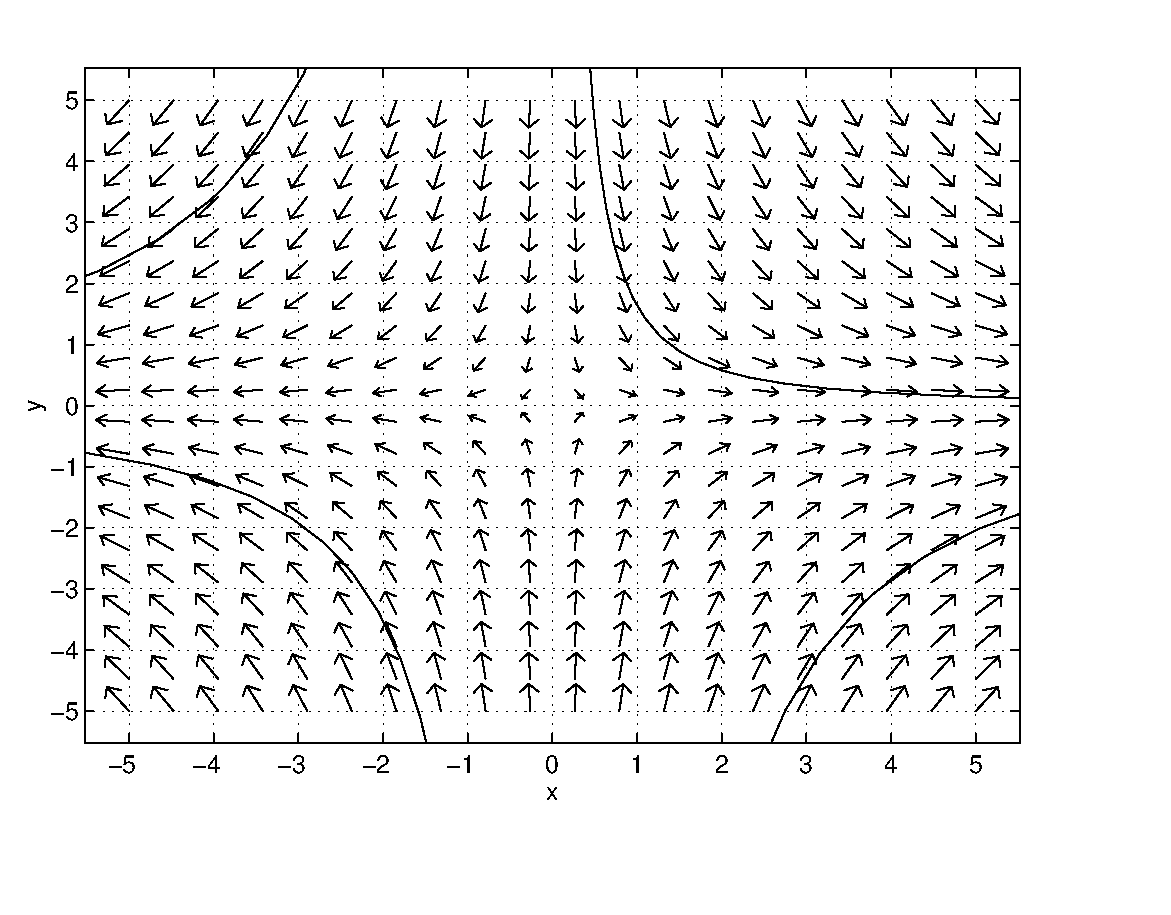
\psfig{file=exfigure/6-3-3a.eps,width=1.8in}
                       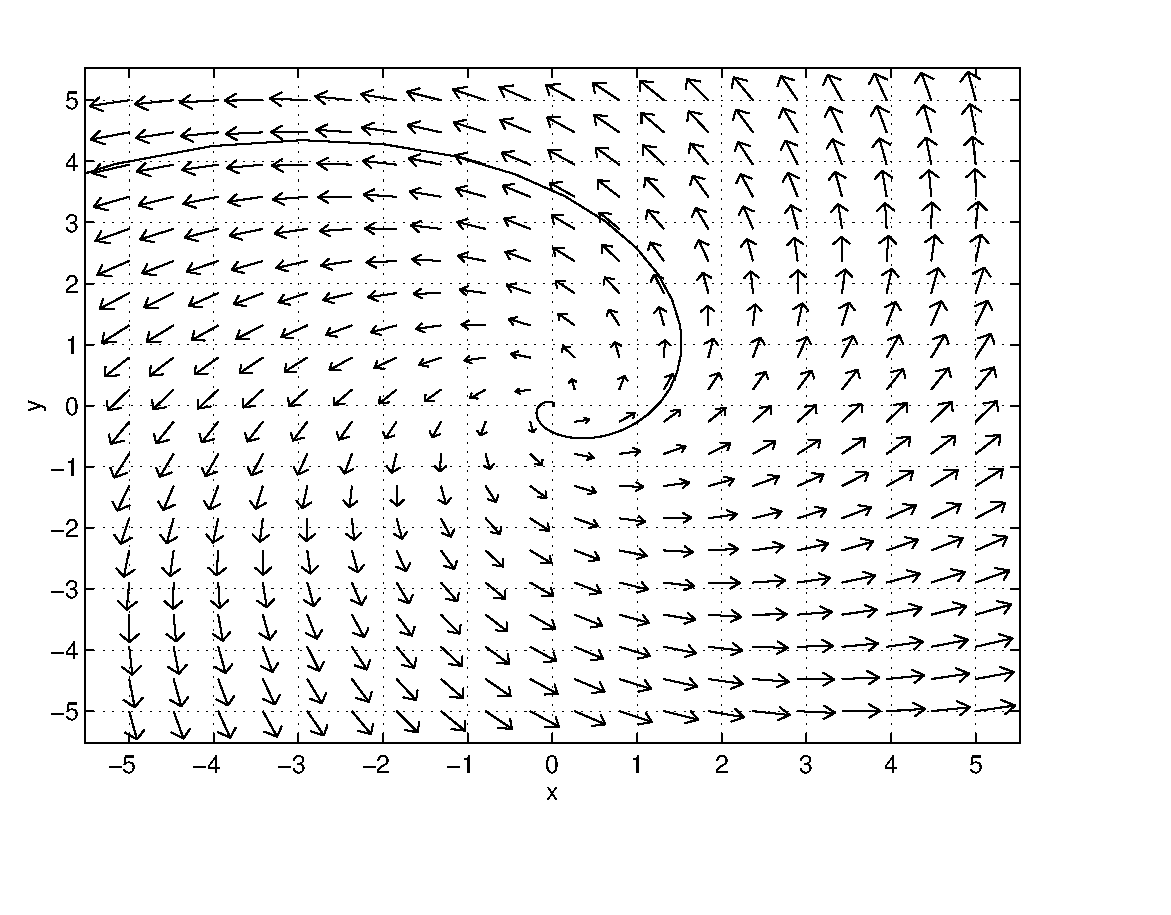
\psfig{file=exfigure/6-3-3b.eps,width=1.8in}
                       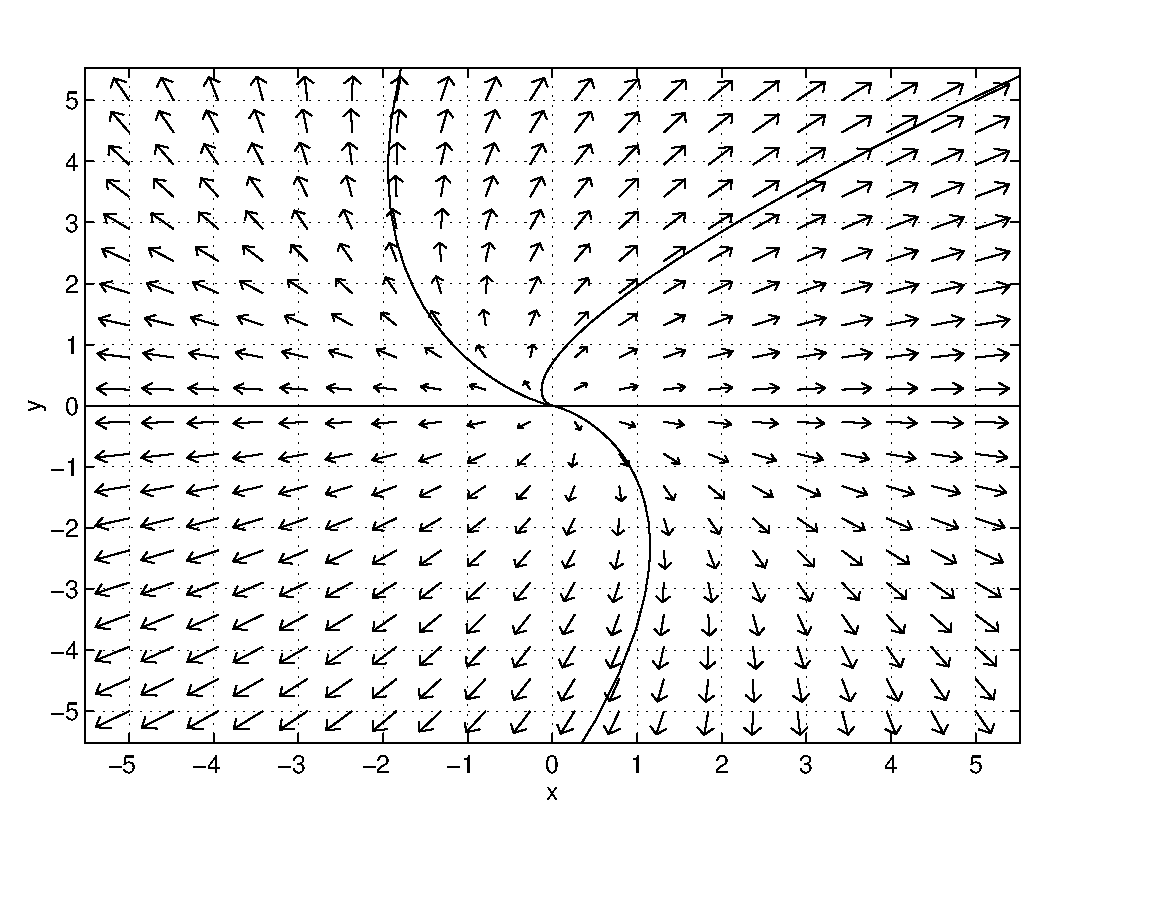
\psfig{file=exfigure/6-3-3c.eps,width=1.8in}}
                \exercapthree{c6.3.3}
\end{figure}
\end{solution}
\end{exercise}

\AEXER

\begin{exercise} \label{a6.3.1}
Use {\pplane} to verify that the nonzero solutions to the system
\[
\frac{dX}{dt} = CX
\]
where
\begin{equation} \label{a6.3.1_C}
C = \Matrix{0 & -1\\ 1 & 0}
\end{equation}
are circles around the origin.  Let 
\[
P = \Matrix{2 & 1\\ 3 & 4}
\]
and  let 
\[
B = P^{-1}CP =  \Matrix{-2.8 & -3.4\\ 2.6 & 2.8}
\]
Describe the solutions to the system
\begin{equation} \label{a6.3.1_B}
\frac{dX}{dt} = BX.
\end{equation}
What is the relationship between solutions of \eqref{a6.3.1_C} to solutions of \eqref{a6.3.1_B}?

\begin{solution}
\soln 

The phase plane 

\begin{figure}[htb]
                       \centerline{%
                       \psfig{file=exfigure/F_6_3_a.eps,width=2.0in}
                       \psfig{file=exfigure/F_6_3_b.eps,width=2.0in}}
                \exercaptwo{a6.3.1}
\end{figure}

\end{solution}
\end{exercise}

\end{document}

%%% Local Variables:
%%% mode: latex
%%% TeX-master: "../linearAlgebra"
%%% End:
